
\section{Bestimmung der IQE bei Raumtemperatur durch Fitting}
\label{chap:grundfitting}
\thispagestyle{fancy}

\begin{figure}[htb]
    \centering
    \begin{minipage}[t]{0.49\linewidth}
        \centering
        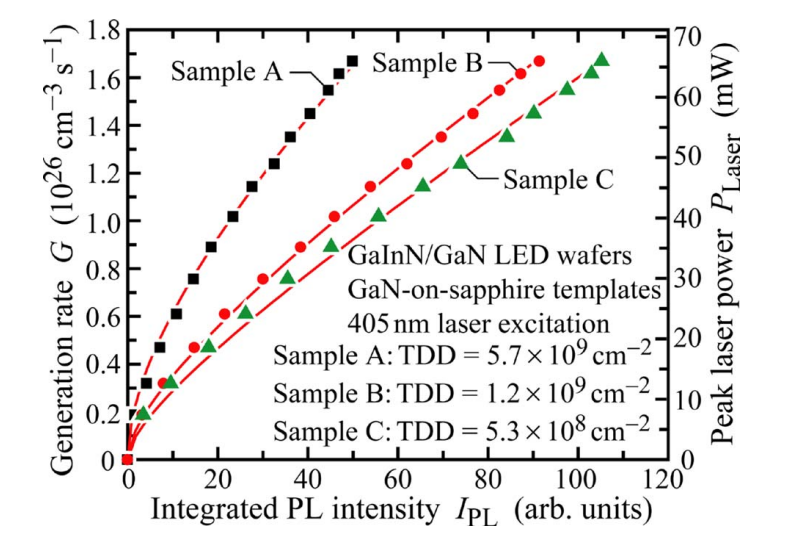
\includegraphics[width=\linewidth]{Bilder/raumtempMethodeBeispielFit.PNG}
        \caption{Fit für die Generationsrate in Abhängigkeit der integrierten PL-Intensität für drei InGaN/GaN MQW Proben mit unterschiedlichen Versetzungsdichten \cite{doi:10.1063/1.3100773}.}
    \end{minipage}% <- sonst wird hier ein Leerzeichen eingefügt
    \hfill
    \begin{minipage}[t]{0.49\linewidth}
        \centering
        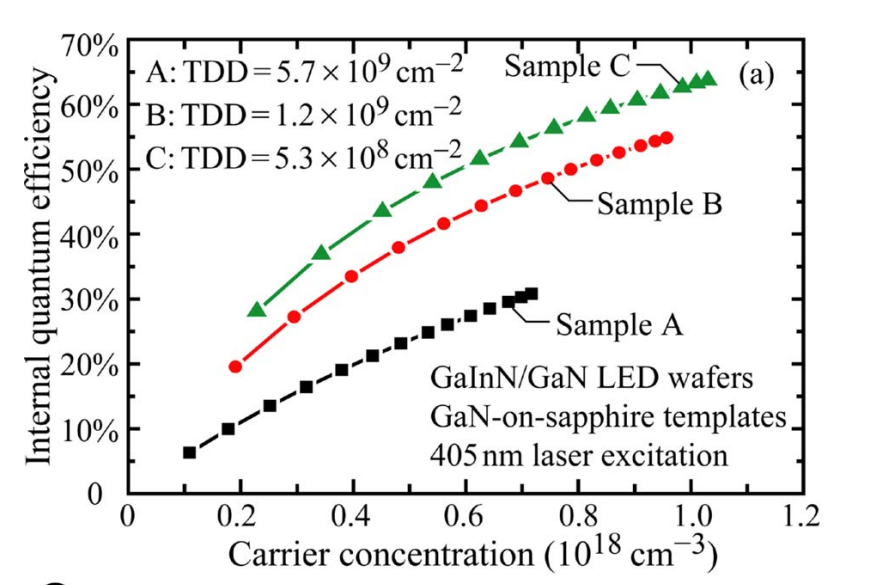
\includegraphics[width=\linewidth]{Bilder/raumtempMethodeIQE.PNG}
        \caption{Ergebnisse für die IQE in Abhängigkeit der Ladungsträgerdichte aus den durch die Fits extrahierten Werte \cite{doi:10.1063/1.3100773}. }
        \label{fig:iqert}
    \end{minipage}
\end{figure}
\noindent
In diesem Kapitel soll nun eine in \cite{doi:10.1063/1.3100773} und \cite{doi:10.1063/1.4917540} gezeigte Methode zur Bestimmung der IQE durch ein Fitting-Modell für die integrierte Intensität in Abhängigkeit der Ladungsträgerdichte vorgestellt werden. Das ist insbesondere von Vorteil, da so ein aufwendiges Runterkühlen nicht mehr notwendig wäre, da die Spektren allein bei Raumtemperatur durch leistungsdichteabhängige Messungen aufgenommen werden könnten. 
\newline
Angefangen mit der Rekombinationsrate geht das Modell davon aus,
dass bei Raumtemperatur die Auger-Rekombination nur bei sehr hohen Anregungsleistungsdichten wegen der kubischen Abhängigkeit der Ladungsträgerdichte $n$ relevant ist. Die Generationsrate G und die IQE bei Gleichgewichtsbedingungen sind somit
\begin{equation}
    G = R_{eff} = A \cdot n + B \cdot n^2
    \label{eq:generationrate}
\end{equation}  
\begin{equation}
    IQE = \frac{B\cdot n^2}{A \cdot n + B \cdot n^2} = \frac{B\cdot n^2}{G}.
    \label{eq:iqe2}
\end{equation}  
G beschreibt namentlich die Rate der Ladungsträger, die durch Bestrahlung mit dem Laser erzeugt werden und entspricht hierbei der effektiven Rekombinationsrate $R_{eff}$.
Die integrierte PL-Intensität lässt sich als 
\begin{equation}
    I_{PL} = \eta \cdot B \cdot n^2
    \label{eq:integint}
\end{equation} 
darstellen. $\eta$ ist eine Konstante, die durch das Volumen der angeregten aktiven Region und der Kollektionseffizienz bestimmt wird. Durch Eliminierung von $n$ in den Gleichungen \ref{eq:generationrate} und \ref{eq:integint} kann die Generationsrate durch die integrierte PL-Intensität als
\begin{equation}
    G = \frac{A}{\sqrt{B\cdot n}}\sqrt{I_{PL}} + \frac{1}{\eta} I_{PL}
    %\label{eq:newgenrate}
\end{equation} 
beschrieben werden. Um dies in Zusammenhang mit dem Experiment zu bringen, kann die Generationsrate mit Nutzung experimenteller Werte getrennt als
\begin{equation}
    G = \frac{P_{laser} (1-R)\alpha l}{A_{spot} l h v} = \frac{P_{laser}(1-R) \alpha }{ (A_{spot} h v)}
   % \label{eq:newgenrate}
\end{equation} berechnet werden.
Dabei ist $P_{laser}$ die optische Leistung, die auf der Probe landet, $R$ ist die Fresnel Reflexion auf der Probenoberfäche, $A_{spot}$ ist die Fläche des Laserspots auf der Probe, $h v$ ist die Energie eines Photons mit $193 nm$ und $\alpha$ ist der Absorptionskoeffizient. Damit ist es möglich die Generationsrate zu bestimmen und in Abhängigkeit der integrierten PL-Intensität darzustellen. Dadurch, dass die Koeffizienten $c_1 = A \sqrt{B  \eta}$ und $c_2 = 1 / \eta$ durch einen Fit der Generationsrate in Abhängigkeit der integrierten Intensität extrahiert werden können, ist es möglich die IQE zu bestimmen. Dazu wird $c_1$ nach A umgestellt ($A = \sqrt{B \eta} \cdot c1$) und in \ref{eq:generationrate} eingesetzt, woraus sich 
\begin{equation}
    G = \sqrt{B \eta} \cdot c_1\cdot n + (\sqrt{B} \cdot n)^2
    \label{eq:generationrateneu}
\end{equation}  
ergibt. 
Durch Lösen von Gleichung \ref{eq:generationrateneu}, für $(\sqrt{B} \cdot n)$ und Einsetzen in Gleichung \ref{eq:iqe2} ist es so möglich die IQE basierend auf anregungsleistungsdichteabhängigen PL-Messungen bei Raumtemperatur zu bestimmen (Abb. \ref{fig:iqert}).


